%versi 2 (8-10-2016)
\chapter{Perancangan}
\label{chap:perancangan}

Bab ini akan menjelaskan mengenai perancangan aplikasi yang dibangun yang merujuk pada hasil studi dan analisis yang telah dibahas pada bab sebelumnya. Pada bab ini juga akan dibahas perancangan interaksi antar node, perancangan antarmuka, perancangan kelas, perancangan masukan dan keluaran aplikasi yang dibangun.

\section{Perancangan Interaksi Antar Node}
\label{sec:skripsi} 
Perancangan Interaksi antar node akan menginformasikan proses interaksi antar node dengan base station dan perangkat lunak yang dibangun untuk pengguna dan admin.

   \subsection{Diagram Sequence "Check Status Node" Aplikasi Pengguna}
   
   \begin{figure}[H]
    	\centering  
    	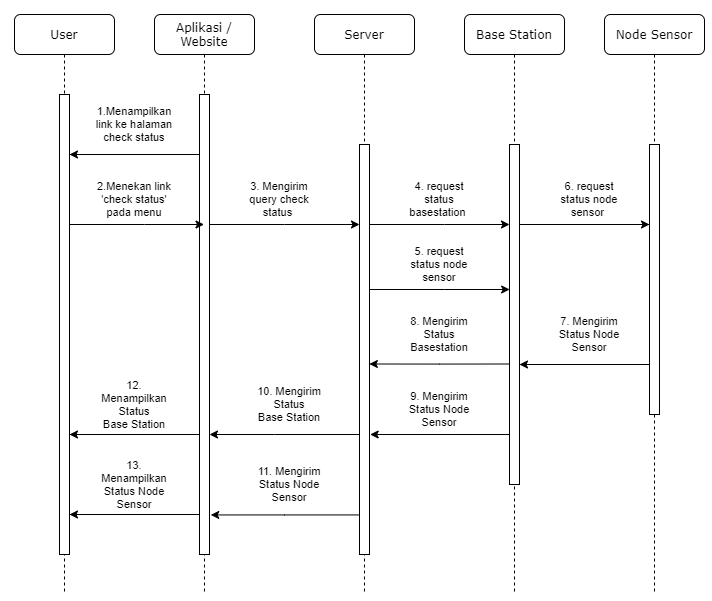
\includegraphics[scale=0.55]{Check_Status_SD(rev).png}  
    	\caption[Sequence Diagram Check Status Aplikasi Pengguna]{Sequence Diagram Check Status Aplikasi Pengguna} 
    	\label{fig:Sequence Diagram Check Status Aplikasi Pengguna} 
    \end{figure}
   
   Pada Check Status Node, pertama aplikasi/website akan menampilkan link ke halaman check status yang berada di header. Selanjutkan \textit{user} dapat menekan link yang ditampilkan tersebut. Aplikasi akan mengirim perintah query yang dikirimkan ketika \textit{user} menekan link check status node, ke server. Server akan menerima query request yang dikirimkan untuk dilanjutkan ke \textit{base station}. \textit{Base station} akan mengirimkan informasi status \textit{base station} dan mengambil status seluruh node yang terhubung dalam jaringan. Ketika seluruh informasi status node diterima oleh \textit{base station}, \textit{base station} akan mengirim kembali informasi tersebut ke server. Server akan menerima seluruh informasi yang dikirimkan oleh \textit{base station} untuk ditampilkan ke aplikasi. Terakhir, aplikasi akan menampilka status terbaru dari setiap node yang terhubung dalam jaringan kepada \textit{user}.
   
   \subsection{Diagram Sequence "Check Status Node" Aplikasi Admin}
   
   \begin{figure}[H]
    	\centering  
    	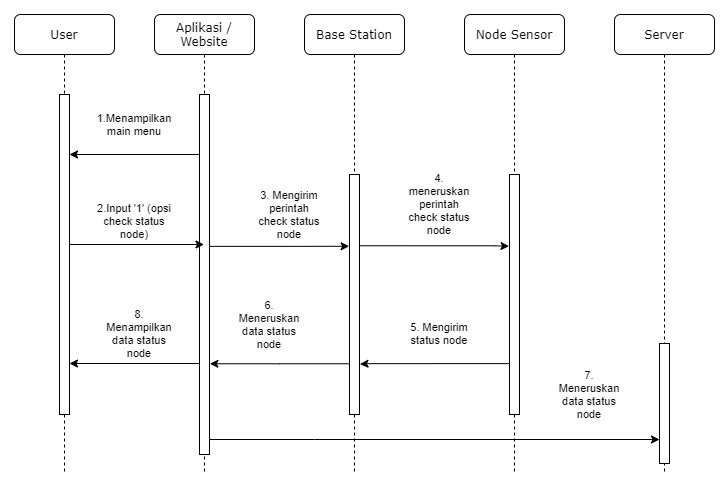
\includegraphics[scale=0.55]{Copy of 2021_seqD_checkStatus_Admin.png}  
    	\caption[Sequence Diagram Check Status Aplikasi Admin]{Sequence Diagram Check Status Aplikasi Admin} 
    	\label{fig:Sequence Diagram Check Status Aplikasi Admin} 
    \end{figure}
    
     Aplikasi admin akan menampilkan opsi fitur yang dapat dipilih oleh pengguna (admin) ketika program pertama kali dieksekusi. Pengguna dapat memilih opsi 'Check Status Node' dengan cara melakukan input '1' pada shell. Setelah pengguna melakukan input, aplikasi admin akan mengirim perintah check status node dari base station ke seluruh node yang terhubung dalam jaringan. Node sensor akan mulai mengirim data status nodenya masing-masing, ke base station. Base station akan menerima data status node tersebut dan meneruskannya ke aplikasi admin untuk ditampilkan ke pengguna. Base station juga akan meneruskan data status node tersebut ke server untuk disimpan. 
   
   \subsection{Diagram Sequence "\textit{Sensing}" Aplikasi Pengguna}
   
   \begin{figure}[H]
    	\centering  
    	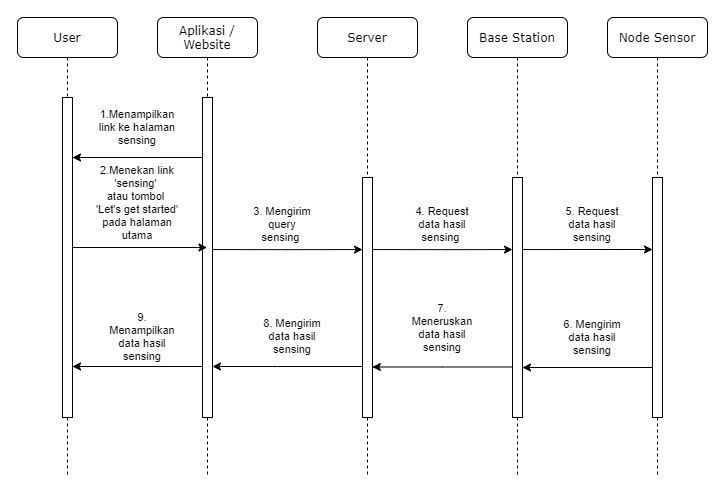
\includegraphics[scale=0.55]{Sensing_SeqD_rev.png}  
    	\caption[Sequence Diagram Sensing Aplikasi Pengguna]{Sequence Diagram Sensing Aplikasi Pengguna} 
    	\label{fig:Sequence Diagram Mulai Sensing Aplikasi Pengguna} 
    \end{figure}
   
   Untuk melakukan \textit{sensing}, pertama aplikasi/website akan menampilkan link untuk ke halaman \textit{sensing} yang berada header atau tombol yang berada di halaman utama dengan nama '\textit{Lets get started}'. \textit{User} menekan link atau tombol yang berada di halaman utama tersebut untuk berpindah halaman ke halaman \textit{sensing}. Aplikasi akan mengirim query ke server yang berfungsi untuk memberikan perintah \textit{sensing}. Server yang menerima query tersebut akan melakukan request ke \textit{base station} untuk melakukan \textit{sensing}. \textit{Base station} akan melanjukan \textit{request} tersebut pada setiap node sensor yang terhubung dalam jaringan. Seluruh node akan melakukan \textit{sensing}, dan mengirimkan data hasil \textit{sensing} ke \textit{base station} secara real time. \textit{Base station} akan mengambil seruruh data hasil \textit{sensing} dari setiap node dan diteruskan ke server. Server akan menyimpan data hasil \textit{sensing} yang dikirimkan oleh \textit{base station} untuk ditampilkan di halaman aplikasi. Aplikasi akan menampilkan data hasil \textit{sensing} yang dikirimkan oleh node sensor dan \textit{base station}.
   
   \subsection{Diagram Sequence "\textit{Mulai Sensing}" Aplikasi Admin}
   
   \begin{figure}[H]
    	\centering  
    	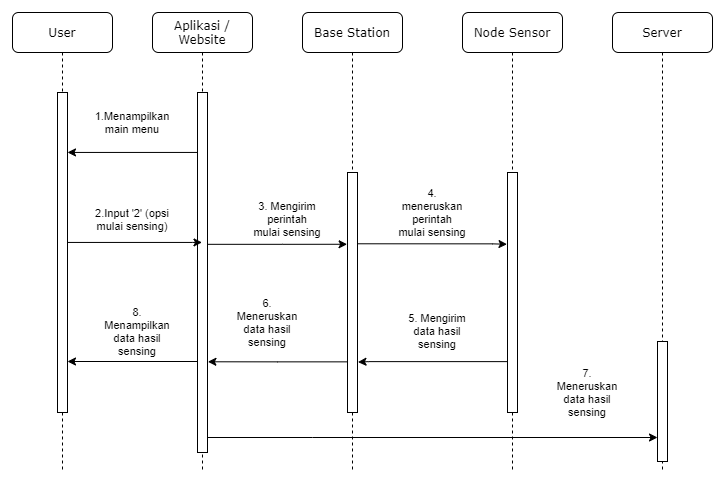
\includegraphics[scale=0.55]{2021_seqD_mulaiSensing_Admin.png}  
    	\caption[Sequence Diagram Sensing Aplikasi Admin]{Sequence Diagram Sensing Aplikasi Admin} 
    	\label{fig:Sequence Diagram Mulai Sensing Aplikasi Admin} 
    \end{figure}
    
    Aplikasi admin akan menampilkan opsi fitur yang dapat dipilih oleh pengguna (admin) ketika program pertama kali dieksekusi. Pengguna dapat memilih opsi 'mulai \textit{sensing}' dengan cara melakukan input '2' pada shell. Setelah pengguna melakukan input, aplikasi admin akan mengirim perintah mulai \textit{sensing} dari base station ke seluruh node yang terhubung dalam jaringan. Node sensor akan mulai mengirim data hasil \textit{sensing}nya ke base station. Base station akan menerima data hasil \textit{sensing} tersebut dan meneruskannya ke aplikasi admin untuk ditampilkan ke pengguna. Base station juga akan meneruskan data hasil \textit{sensing} tersebut ke server untuk disimpan. 
   
   \subsection{Diagram Sequence "Stop \textit{Sensing}" Aplikasi Admin}
   
   \begin{figure}[H]
    	\centering  
    	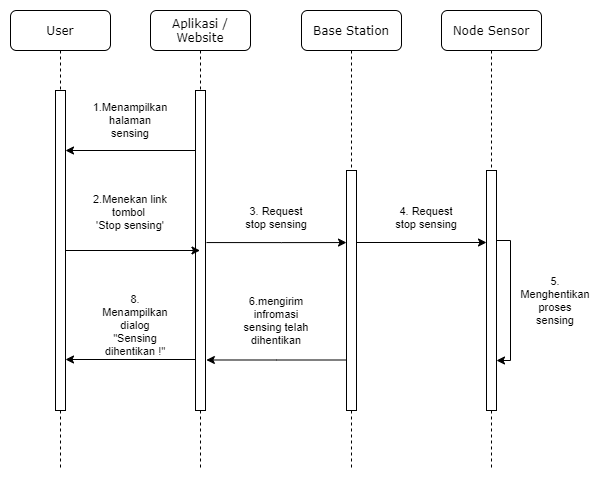
\includegraphics[scale=0.55]{2021_seqD_stopSensing-Page-1.png}  
    	\caption[Sequence Diagram Stop Sensing Aplikasi Admin]{Sequence Diagram Stop Sensing Aplikasi Admin} 
    	\label{fig:Sequence Diagram Stop Sensing Aplikasi Admin} 
    \end{figure}
   
   Untuk melakukan stop \textit{sensing}, pengguna cukup memilih opsi stop \textit{sensing} yang berada di opsi fitur (main menu). Ketika opsi stop \textit{sensing} dipilih oleh \textit{user} dengan cara melakukan input '3', aplikasi akan mengirim perintah dari base station ke seluruh node yang terhubung dalam jaringan. \textit{Base station} akan mengirim perintah untuk menghentikan seluruh proses \textit{sensing} yang dilakukan oleh node sensor yang terhubung dalam jaringan. Setelah seluruh node sensor tidak melakukan \textit{sensing}, \textit{base station} akan mengirimkan informasi pada server bahwa seluruh \textit{sensing} telah dihentikan. Server akan melanjutkan informasi tersebut ke aplikasi, dan aplikasi akan menampilkan dialog "Sensing Dihentikan !"
  
 
  
%\dtext{11-12} 

\section{Perancangan Antarmuka Aplikasi}
\label{sec:latex}

    Terdapat beberapa fungsi pada aplikasi yang dibangun yang memerlukan interaksi pada antarmuka seperti yang disebutkan di-subbab \ref{Analisis Fungsi Aplikasi}. Beberapa fungsi yang memerlukan interaksi pada antarmuka diantaranya adalah fungsi check status node, mulai \textit{sensing}, dan stop \textit{sensing}. Design antarmuka Aplikasi yang dibangun berbasiskan pada antarmuka website. Berikut adalah perancangan antarmuka halaman-halaman untuk aplikasi yang dibangun.
    
    \subsection{Mockup Halaman Utama}
    Pada halaman utama terdapat judul website dan tombol "\textit{Let's get started}". Jika \textit{user} menekan tombol tersebut maka antarmuka website akan diarahkan ke halaman \textit{sensing} secara otomatis, dan \textit{sensing} akan langsung dilakukan. Pada halaman utama juga \textit{user} dapat memilih halaman yang ingin dikunjungi berdasarkan \textit{link} yang tertera pada
    \textit{header}.
    
    \begin{figure}[H]
    	\centering  
    	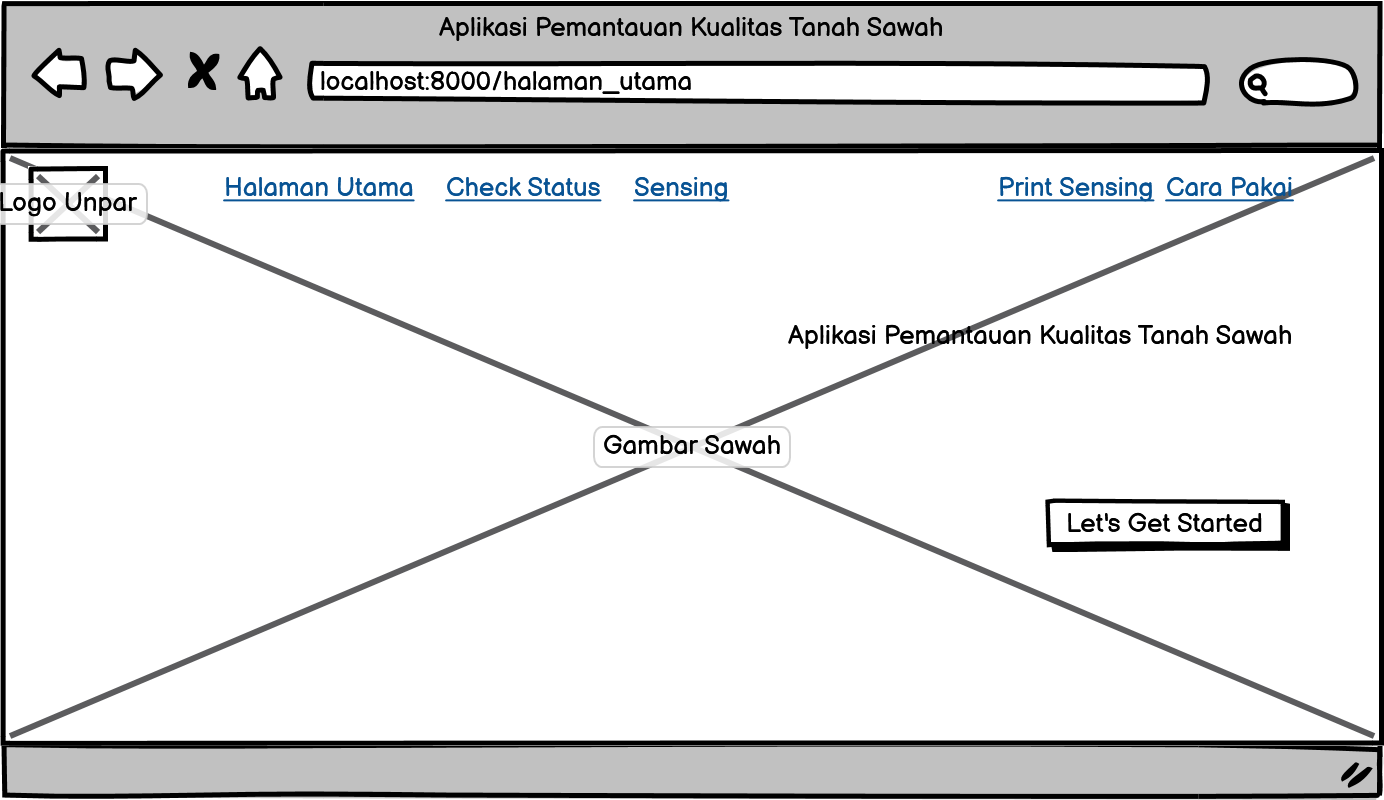
\includegraphics[scale=0.7]{Halaman Utama Mockup.png}  
    	\caption[Mockup Halaman Utama]{Mockup Halaman Utama} 
    	\label{fig:Mockup Halaman Utama} 
    \end{figure}
   
   \subsection{Mockup Halaman "\textit{Sensing}"}
   Halaman \textit{Sensing} memiliki fungsi untuk menampilkan hasil \textit{sensing} yang telah disimpan di basis data secara \textit{real-time}. 
   Sensing secara otomatis akan dilakukan ketika halaman ini dibuka, dan halaman ini akan melakukan \textit{refresh} secara berkala untuk mendapatkan data hasil \textit{sensing} terbaru. Pada halaman ini juga \textit{user} dapat memulai dan menghentikan \textit{sensing}, dengan cara menekan tombol 'mulai sensing' untuk memulai \textit{sensing} atau 'stop \textit{sensing}' untuk menghentikan \textit{sensing}.
   
   \begin{figure}[H]
    	\centering  
    	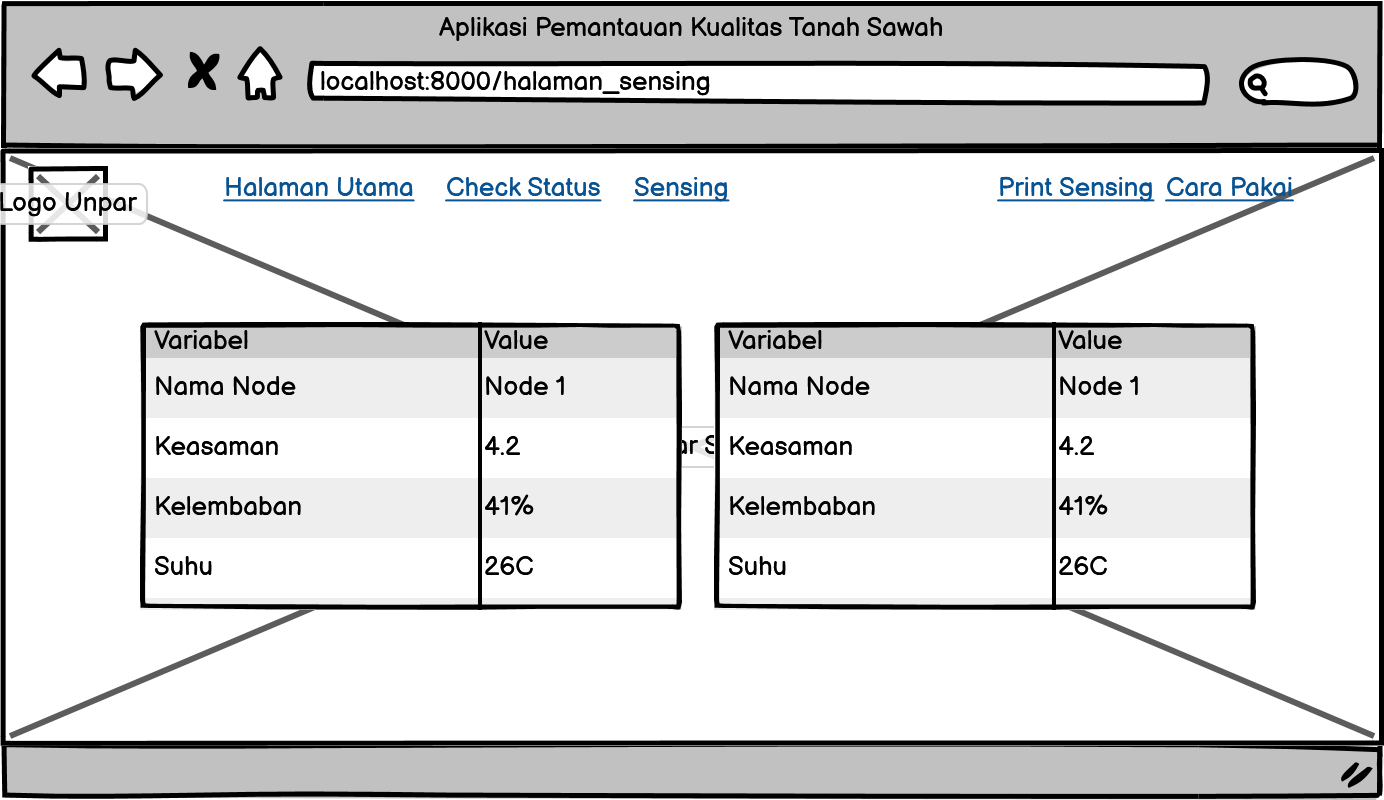
\includegraphics[scale=0.7]{Sensing Mockup.png}  
    	\caption[Mockup Halaman Sensing Online]{Mockup Halaman Sensing Online} 
    	\label{fig:Mockup Halaman Sensing} 
    \end{figure}
   
   
   \subsection{Mockup Halaman "Check Status"}
   Seperti namanya, halaman check status memiliki peran untuk menampilkan status dari setiap node yang disebar. Jika status node aktif maka \textit{value} node pada kolom node tersebut adalah '\textit{Online}'. Sebaliknya jika status node non-aktif maka \textit{value} node pada kolom node tersebut adalah '\textit{Offline}'.
   
   \begin{figure}[H]
    	\centering  
    	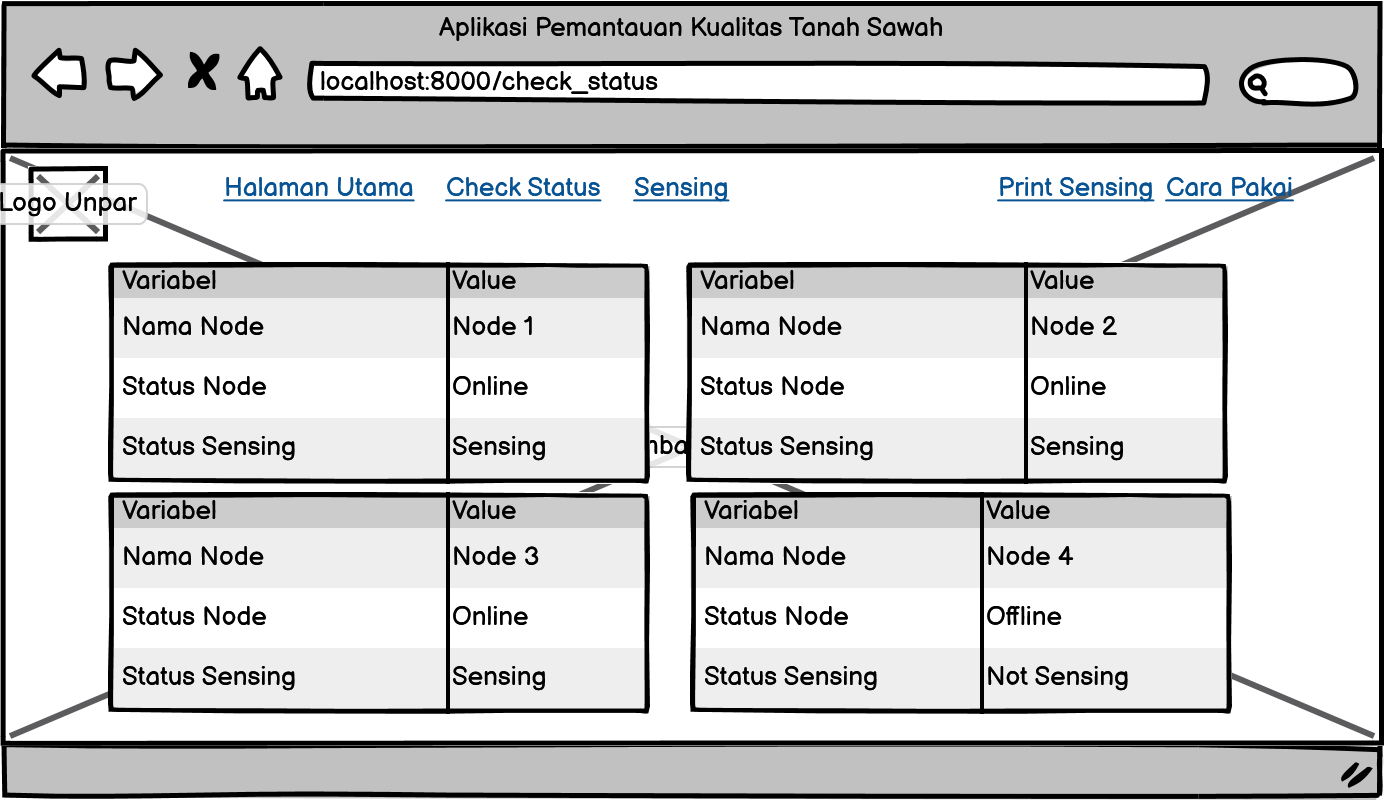
\includegraphics[scale=0.7]{Check Status Mockup.png}  
    	\caption[Mockup Halaman Check Status]{Mockup Halaman Check Status} 
    	\label{fig:Mockup Halaman Check Status} 
    \end{figure}
   
   \subsection{Mockup Halaman "Cara Penggunaan"}
   Halaman cara penggunaan adalah halaman informasi yang menunjukan cara kerja atau pemakaian sistem pemantauan kualitas tanah sawah yang dibangun. Halaman ini meringkas tatacara penggunaan aplikasi agar mudah dimengerti oleh \textit{user}.
   
   \begin{figure}[H]
    	\centering  
    	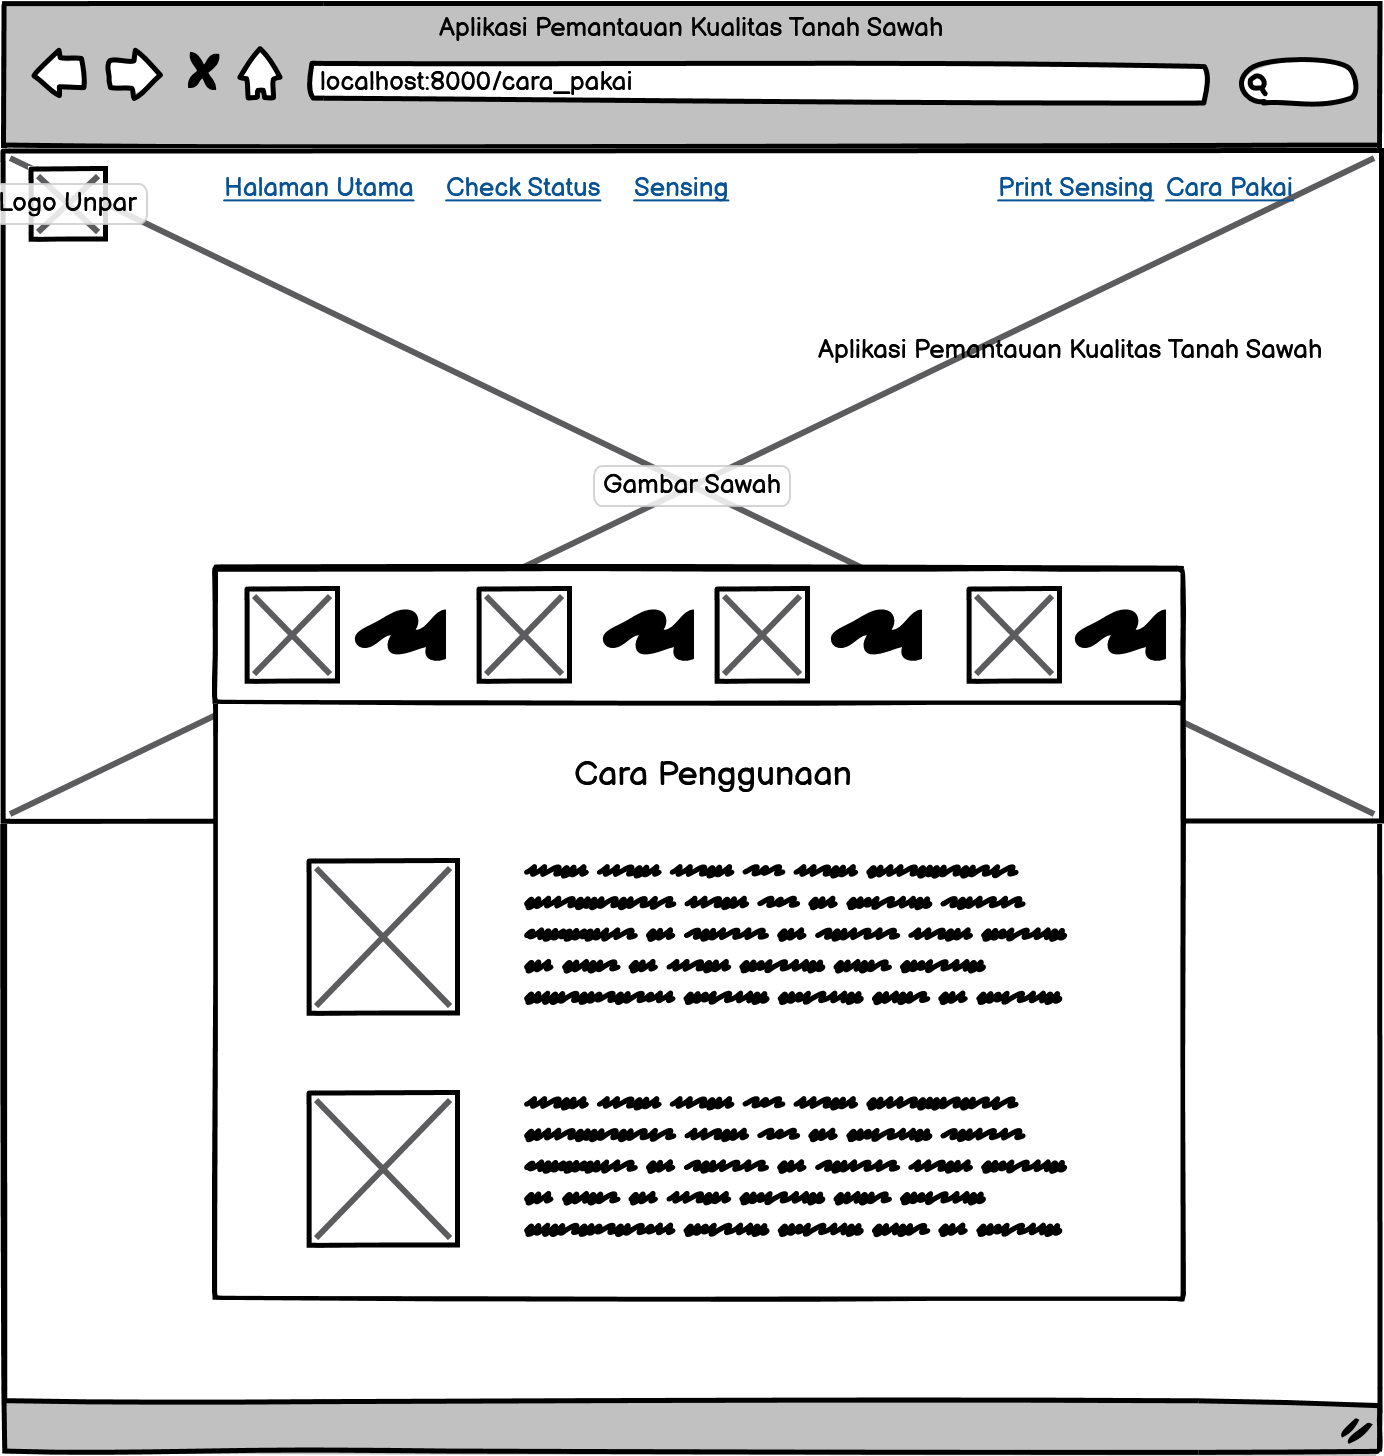
\includegraphics[scale=0.6]{Cara Pakai Mockup.png}  
    	\caption[Mockup Halaman Cara Penggunaan]{Mockup Halaman Cara Penggunaan} 
    	\label{fig:Mockup Halaman Cara Penggunaan} 
    \end{figure}
    
    \subsection{Mockup Halaman "Print Sensing"}
    Halaman "Print Sensing" adalah halaman yang digunakan untuk menampilkan seluruh riwayat \textit{sensing} yang pernah dilakukan. Pengguna juga dapat mencari data riwayat \textit{sensing} tertentu berdasarkan waktu \textit{sensing} maupun kode petak tanah yang dilakukan pengamatan.
    
    \begin{figure}[H]
    	\centering  
    	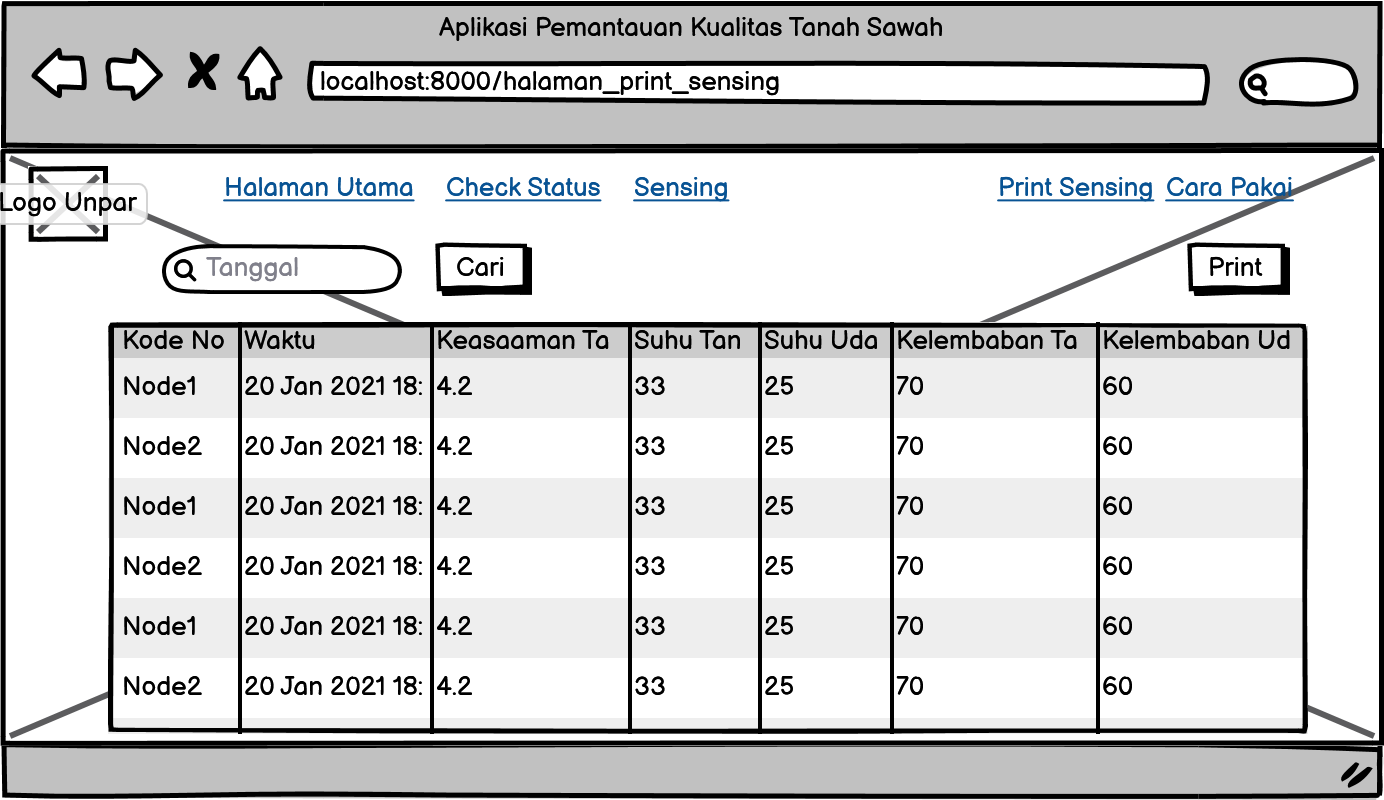
\includegraphics[scale=0.5]{Print Sensing Mockup.png}  
    	\caption[Mockup Halaman Print Sensing]{Mockup Halaman Print Sensing} 
    	\label{fig:Mockup Halaman Print Sensing} 
    \end{figure}
   
%   \subsection{Mockup Halaman "GIS"}
%   Halaman "GIS" adalah halaman yang ditunjukan pada \textit{user} untuk menginformasikan lokasi node berdasarkan koordinat GPS yang terpasang pada perangkat node tersebut.
   
%   \begin{figure}[H]
%     	\centering  
%     	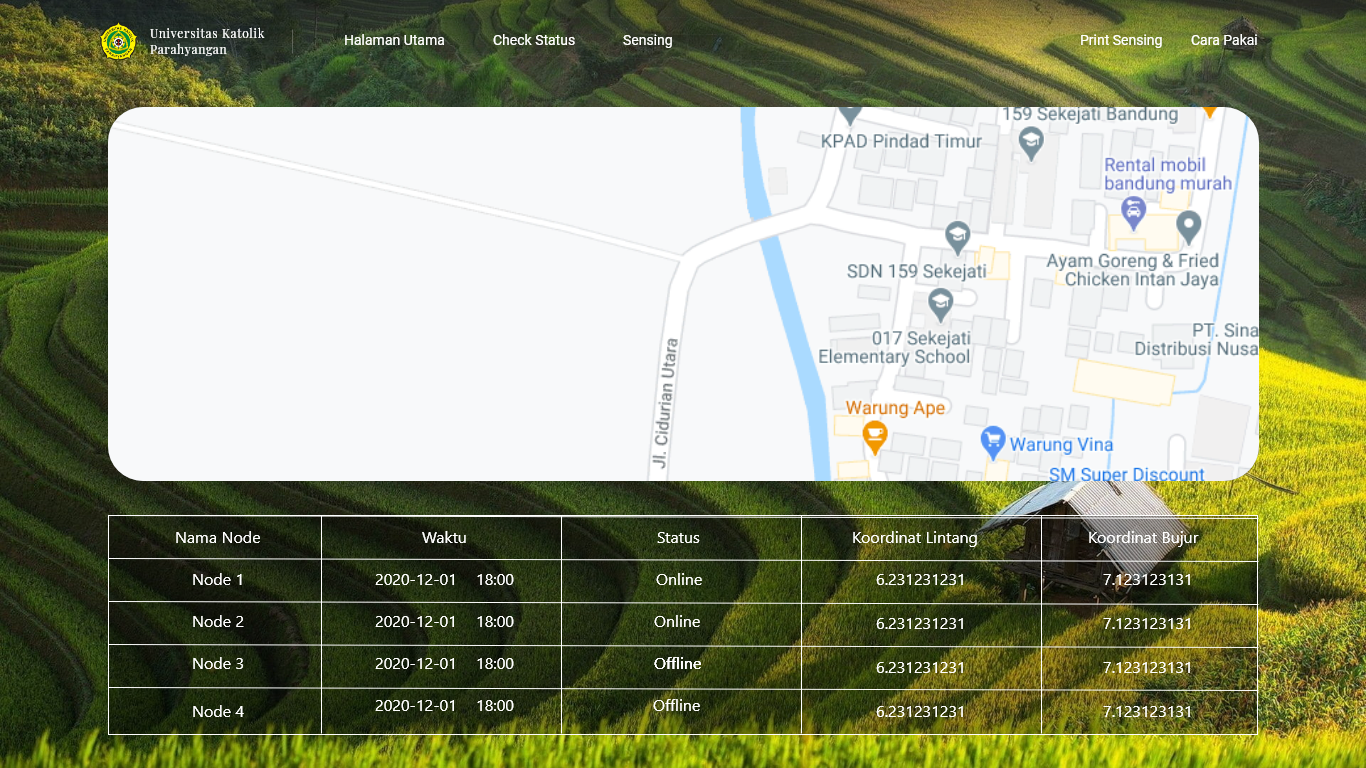
\includegraphics[scale=0.32]{GIS_Proto.png}  
%     	\caption[Mockup Halaman GIS]{Mockup Halaman GIS} 
%     	\label{fig:Mockup Halaman GIS} 
%     \end{figure}

\section{Perancangan Kelas Aplikasi}
    
    Pada subbab ini akan dijelaskan kembali kelas diagram yang terdapat pada aplikasi yang dibangun secara lebih mendetil, yang telah dibahas pada subbab \ref{Analisis Kelas}. Aplikasi yang dibangun memiliki tiga kelas utama yaitu kelas node sensor, kelas sensor \textit{sensing}, dan kelas \textit{base station}.
    
% \subsection{Kelas Sensor Sensing}

%     \begin{figure}[H]
%     	\centering  
%     	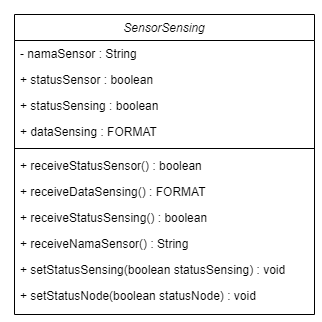
\includegraphics[scale=0.52]{sensor_sensing_cd.png}
%     	\caption[Kelas Diagram Sensor \textit{Sensing}]{Kelas Diagram Sensor \textit{Sensing}} 
%     	\label{fig:Kelas Diagram Sensor Sensing} 
%     \end{figure}
    
%     Kelas Sensor \textit{Sensing} mempresentasikan sensor \textit{sensing} berserta atribut dan fungsinya yang terhubung dengan node sensor.Atribut- atribut yang ada pada kelas ini adalah sebagai berikut:
    
%     \begin{itemize}
%         \item private String namaSensor
        
%         Atribut namaSensor berperan untuk mengidentifikasi sensor yang melakukan sensing berdasarkan namanya
        
%         \item public boolean statusSensor
        
%         Atribut statusSensor berperakn untuk menunjukan status keaktifan sensor
        
%         \item public boolean statusSensing
        
%         Atribut statusSensing berperan untuk menunjukan status sensing yang dilakukan oleh sensor
        
%         \item public FORMAT dataSensing
        
%         Atribut dataSensing berperan sebagai atribut yang menyimpan nilai data yang didapatkan dari hasil sensing oleh sensor
        
%     \end{itemize}
     
%     Methods yang ada pada kelas node sensor adalah sebagai berikut:
    
%     \begin{itemize}
%         \item public boolean receiveStatusSensor
        
%         Method receiveStatusSensor berfungsi untuk mendapatkan status keaktifan sensor
        
%         \item public String receiveDataSensing
        
%         Method receiveDataSensing berfungsi untuk mendapatkan data sensing yang dilakukan oleh sensor
        
%         \item public String receiveStatusSensing
        
%         Method receiveStatusSensing berfungsi untuk mendapatkan status kondisi sensing oleh sensor
        
%         \item public String receiveNamaSensor
        
%         Method receiveNamaSensor berfungsi untuk mengembalikan nama dari sensor yang melakukan sensing
        
%         \item public void setStatusSensing
        
%         Method setStatusSensing berfungsi untuk mengubah nilai dari atribut status sensing. Jika status sensing bernilai false, nilai tersebut mengindikasikan sensor tidak sedang melakukan sensing. Jika status sensing bernilai \textit{true}, maka sensor sedang melakukan sensing.
        
        
%     \end{itemize} 
     
\subsection{Kelas Node Sensor}

    \begin{figure}[H]
    	\centering  
    	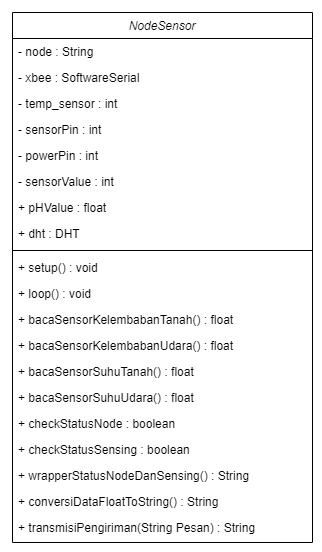
\includegraphics[scale=0.52]{Class_Diagram_Node_Sensor_Fixed.png}
    	\caption[Kelas Diagram Node Sensor]{Kelas Diagram Node Sensor} 
    	\label{fig:Kelas Diagram Node Sensor} 
    \end{figure}
    
    Kelas node sensor memodelkan atribut-atribut yang dimiliki oleh node sensor dan fungsi-fungsi yang dapat dilakukan oleh node sensor. 
    Atribut- atribut yang ada pada kelas ini adalah sebagai berikut:
    
    \begin{itemize}
        \item private String node
        
        Atribut node berperan untuk mengidentifikasi node yang melakukan \textit{sensing} berdasarkan namanya
        
        \item private SoftwareSerial xbee
        
        Atribut xbee berperan sebagai penghubung antara perangkat xbee dengan pin yang terdapat pada perangkat arduino. Atribut ini juga berfungsi sebagai instansiasi pin yang terhubung sebagai recevier dan transivier.
        
        \item private int temp\_sensor
        
        Atribut temp\_sensor memiliki peran untuk menginformasikan letak pin yang digunakan untuk melakukan pengiriman data hasil \textit{sensing} temperatur dan kelembaban tanah.
        
        \item private int sensorPin
        
        Atribut sensorPin merupakan atribut yang berfungsi untuk menginformasikan pin analog yang akan digunakan oleh sensor \textit{sensing} kelembaban tanah.
        
        \item private int powerPin
        
        Atribut powerPin berfungsi untuk mengubah pin tertentu menjadi VCC atau pengganti daya 5V.
        
        
        \item private int sensorValue
        
        Atribut sensorValue berperan sebagai inialisasi data hasil \textit{sensing} yang akan dikonversi dari Analog menjadi Digital untuk sensor \textit{sensing} keasaman tanah.
        
        \item public float pHValue
        
        Atribut pHValue merupakan atribut yang berfungsi sebagai instansiasi nilai pH tanah dan juga atribut penyimpan data hasil \textit{sensing} keasaman tanah.
        
        
        \item DHT dht
        
        Atribur dht adalah atribut intansiasi kelas DHT yang berfungsi untuk menginformasikan pin yang digunakan untuk mengaktifasi senson \textit{sensing} suhu dan kelembaban udara.
        
        % \item TinyGPS gps
        
        % Atribut gps merupakan atribut yang digunakan untuk mengintansiasi kelas TinyGPS, yang akan digunakan untuk mendapatkan koordinat sebaran node.
        
        
    \end{itemize}
    
    Methods yang ada pada kelas node sensor adalah sebagai berikut:
    
    \begin{itemize}
        \item void setup()
        
        Seperti yang telah dibahas pada subbab \ref{void setup}, method setup merupakan method default yang ada ketika membangun program berbasis arduino. Method ini digunakan untuk menginialisasi seluruh atribut termasuk frekuensi komunikasi serial yang akan digunakan. Method ini juga merupakan method pertama yang akan dieksekusi ketika program dijalankan.
        
        \item void loop()
        
        Method loop juga merupakan method default untuk pembangunan program berbasis arduino. Method loop akan dieksekusi secara terus menerus sampai perangkat akhirnya kehabisan daya atau tidak menerima daya. Method loop pada pembangunan aplikasi ini berperan sebagai wrapper yang membungkus method-method lain sebelum dikirimkan ke \textit{base station}. Method loop juga akan menampilkan data hasil \textit{sensing} apabila perangkat arduino terhubung dengan laptop. 
        
        \item public float bacaSensorKelembabanTanah()
        
        Method bacaSensorKelembabanTanah adalah method yang memiliki fungsi untuk melakukan pengambilan data hasil \textit{sensing} yang dilakukan oleh sensor \textit{sensing} kelembaban tanah. Method ini juga melakukan konversi data dari Analog menjadi Digital. Konversi dilakukan karena perangkat sensor \textit{sensing} menggunakan arus daya untuk mengukur kelembaban suatu tanah. Sehingga data yang diterima harus dikonversi terlebih dahulu agar mendapatkan data yang valid.
        
        \item public float bacaSensorSuhuUdara()
        
        Method bacaSensorSuhuUdara berfungsi untuk mengambil dan mengembalikan data suhu udara, hasil \textit{sensing} sensor \textit{sensing} yang terhubung dengan perangkat arduino (node sensor).
        
        \item public float bacaSensorKelembabanUdara()
        
        Method bacaSensorSuhuUdara memiliki fungsi yang sama dengan method bacaSensorSuhuUdara. Namun data yang diambil dan dikembalikan oleh method ini adalah data kelembaban udara.
        
        \item public float bacaSensorSuhuTanah()
        
        Method bacaSensorSuhuTanah berperan untuk melakukan \textit{sensing} terhadap suhu tanah yang dilakukan pengamatan. Method ini juga akan mengembalikan nilai suhu tahan dari hasil \textit{sensing} yang dilakukan.
        
        \item public float bacaSensorPHtanah()
        
        Seperti method bacaSensorKelembabanTanah, method bacaSensorPHtanah perlu melakukan konversi data hasil \textit{sensing}. Namun, untuk method ini data yang perlu dikonversi adalah data keasaaman tanah yang dilakukan oleh perangkat \textit{sensing} pH tanah.
        
        \item public boolean checkStatusNode()
        
        Method checkStatusNode berfungsi untuk menginformasikan status keaktifan node. Method akan mengembalikan nilai \textit{true} apabila node aktif (\textit{online}), dan akan mengembalikan nilai \textit{false} apabila node tidak aktif (\textit{offline}).
        
        \item public boolean checkStatusSensing()
        
        Method checkStatusSensing memiliki fungsi untuk menginformasikan status \textit{sensing} dari node sensor. Apabila sensor sedang melakukan \textit{sensing} maka method akan mengembalikan nilai \textit{true}. Namun juka sensor tidak melakukan \textit{sensing} maka method akan mengembalikan nilai \textit{false}.
        
        \item public String wrapperStatusNodeDanSensing()
        
        Method wrapperStatusNodeDanSensing berfungsi sebagai method pembukungkus antara method checkStatusNode dan checkStatusSensing. Method ini dibuat agar program dapat ditulis dengan rapi dan mudah untuk dimengerti. Selain itu method checkStatusNode dan checkStatusSensing merupakan method yang berhubungan langsung dengan perangkat node sensor.
        
        \item public String conversiDataFloatToString()
        
        Untuk dapat mengirimkan data tersebut menggunakan xbee, maka seluruh tipe data hasil \textit{sensing} harus dikonversi terlebih dahulu dari float menjadi string. Setelah data telah dikonversi maka hasil konversi akan dimasukan kedalam parameter method transmisiPengiriman untuk dikirimkan ke \textit{base station}.
        
        \item public String transmisiPengiriman(String pesan)
        
        Method transmisiPengiriman merupakan method terakhir yang akan dieksekusi didalam method loop. Method ini bertanggung jawab dalam pengiriman hasil pesan yang telah dikonversi ke \textit{base station}. Setelah method ini dieksekusi, maka proses loop (melakukan \textit{sensing} berikutnya) baru kembali dilakukan.
        
        % \item displayInfoGIS()
        
        % Method displayInfoGIS digunakan untuk mendapatkan koordinat lintang dan bujur dari posisi node yang terhubung.  
        
    \end{itemize}

\subsection{Kelas Base Station}

    \begin{figure}[H]
    	\centering  
    	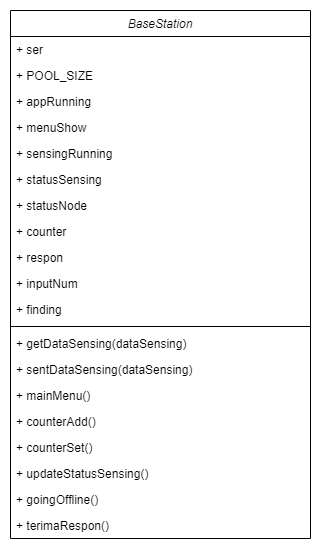
\includegraphics[scale=0.52]{Basestation_CD_FINAL_BAB4.png}
    	\caption[Kelas Diagram \textit{Base station}]{Kelas Diagram \textit{Base station}} 
    	\label{fig:Kelas Diagram Base Station} 
    \end{figure}
    
     Kelas \textit{Base station} mempresentasikan atribut dan fungsi SINK terhubung dengan node sensor dalam jaringan.Atribut- atribut yang ada pada kelas ini adalah sebagai berikut:

    \begin{itemize}
        \item ser
        
        Atribut ser berfungsi sebagai inialisasi pin yang menjadi penghubung antar perangkat Raspberry Pi dengan perangkat XBee. Artibut ini juga menginstansiasi \textit{port} (pin) yang terhubung dengan xbee, berserta frekuensi komunikasi serial yang digunakan agar dapat bertukar pesan dengan node sensor.  
        
        \item POOL\_SIZE
        
        Atribut POOL\_SIZE berperan sebagai atribut penampung yang menginformasikan banyaknya node yang terhubung dalam jaringan. Atribut ini akan digunakan dalam \textit{thread} agar data yang dikirim oleh node dapat diterima, walaupun data diterima dalam waktu bersamaan.
        
        \item appRunning
        
        Atribut appRunning digunakan untuk menginialisasi kondisi \textit{loop} yang dieksekusi pertama kali ketika program dieksekusi. Atribut appRunning akan terus bernilai \textit{True} selama tidak ada interrupt dari keyboard. Selama appRunning bernilai \textit{True} maka program akan terus dieksekusi didalam \textit{loop}.
        
        \item menuShow
        
        Sama seperti appRunning, menuShow berperan untuk menginialisasi kondisi \textit{loop}. Namun menuShow digunakan didalam \textit{loop} appRunning, yang memiliki fungsi untuk terus menampilkan opsi fitur aplikasi \textit{base station} (\textit{main menu}) ketika suatu perintah telah di eksekusi.
        
        \item sensingRunning
        
        SensingRunning juga berperan sebagai inialisasi dari suatu kondisi loop. Namun, SensingRunning digunakan khusus untuk melakukan \textit{loop} \textit{sensing} secara terus menerus, sehingga data hasil \textit{sensing} yang dikirimkan oleh node sensor dapat diterima dan tampilkan pada \textit{shell} aplikasi.
        
        
        \item statusSensing
        
        Atribut statusSensing digunakan untuk menampung nilai status pengamatan yang dikirimkan oleh node sensor. Status bernilai '\textit{True}' jika sensor sedang melakukan \textit{sensing}, dan bernilai '\textit{False}' jika sebaliknya. 
        
        
        \item statusNode
        
        Seperti statusSensing, status node juga digunakan untuk menampung nilai. Namun nilai yang ditampung dalam atribut ini adalah status keaktifan node. Jika node berstatus '\textit{Online}' maka nilai dari status node adalah '\textit{True}', begitupula sebaliknya jika node berstatus '\textit{Offline}' maka nilai dari status node adalah '\textit{False}'.
        
        \item counter
        
        Atribut counter digunakan sebagai nilai penghitung batas waktu tunggu respon dari node ketika \textit{base station} telah mengirim perintah.
        
        \item respon
        
        Atribut respon digunakan sebagai atribut yang menampung jumlah node yang merespon ketika \textit{base station} mengirim perintah.
        
        \item inputNum
        
        Atribut inputNum berfungsi untuk menampung nilai dari \textit{input} yang dimasukan oleh Admin. Nilai dari atribut ini yang akan digunakan untuk memilih opsi instruksi dari fitur yang akan dieksekusi.
        
        \item finding
        
        Atribut finding digunakan untuk menampung nilai dari status sensing yang didapatkan dari respon node sensor dari perintah 'stop sensing' oleh base station. 
        

    \end{itemize}
    
    Methods yang ada pada kelas node sensor adalah sebagai berikut:
    
    \begin{itemize}
        \item getDataSensing(dataSensing)
        
        Method getDataSensing berfungsi untuk mendapatkan seluruh data hasil \textit{sensing} yang dikirimkan oleh masing-masing node yang terhubung dalam jaringan
        
        
        \item sentDataSensing(dataSensing)
        
        Method sentDataSensing berfungsi untuk mengirim seluruh data yang telah diterima oleh \textit{base station} ke server
        
        \item mainMenu
        
        Method mainMenu berfungsi untuk menampilkan daftar opsi fitur yang dapat dipilih oleh admin untuk mengirim perintah ke node sensor dari \textit{base station}
        
        \item counterAdd
        
        Method counterAdd berfungsi untuk menambahkan nilai atribut counter juga untuk membatasi waktu tunggu respon node sensor setelah \textit{base station} mengirim perintah
        
        \item counterSet
        
        Method counterSet berfungsi untuk melakukan \textit{reset} pada nilai atribut counter setelah batas waktu tunggu respon node sensor habis.
        
        \item updateStatusSensing
        
        Method updateStatusSensing berperan untuk melakukan \textit{update} terhadap basis data ketika status sensing diterima oleh \textit{base station}.
        
        \item goingOffline
        
        Method goingOffline digunakan untuk melakukan \textit{update} terhadap basis data ketika aplikasi base station dimatikan.
        
        \item terimaRespon
        
        Method terimaRespon berperan untuk menghitung jumlah node yang membalas atau merespon ketika \textit{base station} telah mengirim perintah
        
    \end{itemize}

\section{Perancangan \textit{Input} dan \textit{Output}}
Aplikasi ini berbasis website sehingga menggunakan \textit{button} pada halaman untuk menerima \textit{input} dan tabel pada halaman untuk menampilkan data. Aplikasi yang dibangun juga memiliki dua halaman dengan fungsi yang berbeda-beda sebagai fungsi utama. Halaman yang dimaksud adalah halaman \textit{sensing} dan halaman check status node. Pada halaman 'Sensing' \textit{user} dapat menekan tombol mulai \textit{sensing} untuk memulai \textit{sensing} pada tanah yang diuji. Pada halaman \textit{sensing} juga, \textit{user} dapat melakukan aktifitas hentikan \textit{sensing} dengan menekan tombol 'stop \textit{sensing}'. Untuk menampilkan status setiap node, \textit{user} dapat menekan link yang merujuk pada halaman check status node, dan aplikasi akan menampilkan status dari setiap node yang terhubung dalam jaringan. 


% \label{sec:latex}
% Berikut adalah contoh pembuatan tabel. 
% Penempatan tabel dan gambar secara umum diatur secara otomatis oleh \LaTeX{}, perhatikan contoh di file bab2.tex untuk melihat bagaimana cara memaksa tabel ditempatkan sesuai keinginan kita.

% Perhatikan bawa berbeda dengan penempatan judul gambar gambar, keterangan tabel harus diletakkan di atas tabel!!
% Lihat Tabel~\ref{tab:contoh1} berikut ini:

% \begin{table}[H] %atau h saja untuk "kira kira di sini"
% 	\centering 
% 	\caption{Tabel contoh}
% 	\label{tab:contoh1}
% 	\begin{tabular}{cccc}
% 		\toprule
% 		& $v_{start}$ & $\mathcal{S}_{1}$ & $v_{end}$\\

% 		\midrule
% 		$\tau_{1}$ & 1 & 12& 20\\
% 		$\tau_{2}$ & 1 &  & 20\\
% 		$\tau_{3}$ & 1 & 9 & 20\\
% 		$\tau_{4}$ & 1 &  & 20\\

% 		\bottomrule
		
% 	\end{tabular} 
% \end{table}
% Tabel~\ref{tab:cthwarna1} dan Tabel~\ref{tab:cthwarna2} berikut ini adalah tabel dengan sel yang berwarna dan ada dua tabel yang bersebelahan. 
% \begin{table}[H]
% 	\begin{minipage}[c]{0.49\linewidth}
% 		\centering
% 		\caption{Tabel bewarna(1)}
% 		\label{tab:cthwarna1}
% 		\begin{tabular}{ccccc}
% 			\toprule
% 			 & $v_{start}$ & $\mathcal{S}_{2}$ & $\mathcal{S}_{1}$ & $v_{end}$\\
			
% 			\midrule
% 			$\tau_{1}$ & 1 & 5 \cellcolor{green}& 12& 20\\
% 			$\tau_{2}$ & 1 & 8 \cellcolor{green}& & 20\\
% 			$\tau_{3}$ & 1 & 2/8/17 \cellcolor{green}& 9 & 20\\
% 			$\tau_{4}$ & 1 & \cellcolor{red}& & 20\\
			
% 			\bottomrule

% 		\end{tabular}
% 	\end{minipage}
% 	\begin{minipage}[c]{0.49\linewidth}
		
% 		\centering 
% 		\caption{Tabel bewarna(2)}
% 		\label{tab:cthwarna2}
% 		\begin{tabular}{ccccc}
% 			\toprule
% 			 & $v_{start}$ & $\mathcal{S}_{1}$ & $\mathcal{S}_{2}$ & $v_{end}$\\
			
% 			\midrule
% 			$\tau_{1}$ & 1 & 12& 5 \cellcolor{red} &20\\
% 			$\tau_{2}$ & 1 &  &  8 \cellcolor{green} &20\\
% 			$\tau_{3}$ & 1 & 9 & 2/8/17 \cellcolor{green} &20\\
% 			$\tau_{4}$ & 1 &   & \cellcolor{red} &20\\
			
% 			\bottomrule
		
% 		\end{tabular}
% 	\end{minipage}
% \end{table}

% \section{Kutipan}
% \label{subs:kutipan} 
% Berikut contoh kutipan dari berbagai sumber, untuk keterangan lebih lengkap, silahkan membaca file referensi.bib yang disediakan juga di template ini.
% Contoh kutipan:
% \begin{itemize}
% 	\item Buku:~\cite{berg:08:compgeom} 
% 	\item Bab dalam buku:~\cite{kreveld:04:GIS}
% 	\item Artikel dari Jurnal:~\cite{buchin:13:median}
% 	\item Artikel dari prosiding seminar/konferensi:~\cite{kreveld:11:median}
% 	\item Skripsi/Thesis/Disertasi:~\cite{lionov:02:animasi}~\cite{wiratma:10:following}~\cite{wiratma:22:later}
% 	\item Technical/Scientific Report:~\cite{kreveld:07:watertight}
% 	\item RFC (Request For Comments):~\cite{RFC1654}
% 	\item Technical Documentation/Technical Manual:~\cite{Z.500}~\cite{unicode:16:stdv9}~\cite{google:16:and7}
% 	\item Paten:~\cite{webb:12:comm}
% 	\item Tidak dipublikasikan:~\cite{wiratma:09:median}~\cite{lionov:11:cpoly}
% 	\item Laman web:~\cite{erickson:03:cgmodel}  
% 	\item Lain-lain:~\cite{agung:12:tango}
% \end{itemize}    
  
% \subsection{Gambar}

% Pada hampir semua editor, penempatan gambar di dalam dokumen \LaTeX{} tidak dapat dilakukan melalui proses {\it drag and drop}.
% Perhatikan contoh pada file bab2.tex untuk melihat bagaimana cara menempatkan gambar.
% Beberapa hal yang harus diperhatikan pada saat menempatkan gambar:
% \begin{itemize}
% 	\item Setiap gambar {\bf harus} diacu di dalam teks (gunakan {\it field} {\sc label})
% 	\item {\it Field} {\sc caption} digunakan untuk teks pengantar pada gambar. Terdapat dua bagian yaitu yang ada di antara tanda $[$ dan $]$ dan yang ada di antara tanda $\{$ dan $\}$. Yang pertama akan muncul di Daftar Gambar, sedangkan yang kedua akan muncul di teks pengantar gambar. Untuk skripsi ini, samakan isi keduanya.
% 	\item Jenis file yang dapat digunakan sebagai gambar cukup banyak, tetapi yang paling populer adalah tipe {\sc png} (lihat Gambar~\ref{fig:ularpng}), tipe {\sc jpg} (Gambar~\ref{fig:ularjpg}) dan tipe {\sc pdf} (Gambar~\ref{fig:ularpdf})
% 	\item Besarnya gambar dapat diatur dengan {\it field} {\sc scale}.
% 	\item Penempatan gambar diatur menggunakan {\it placement specifier} (di antara tanda  $[$ dan $]$ setelah deklarasi gambar.
% 	Yang umum digunakan adalah {\bf H} untuk menempatkan gambar {\bf sesuai} penempatannya di file .tex atau  {\bf h} yang berarti "kira-kira" di sini. \\
% 	Jika tidak menggunakan {\it placement specifier}, \LaTeX{} akan menempatkan gambar secara otomatis untuk menghindari bagian kosong pada dokumen anda.
% 	Walaupun cara ini sangat mudah, hindarkan terjadinya penempatan dua gambar secara berurutan. 	
% 	\begin{itemize}
% 		\item Gambar~\ref{fig:ularpng} ditempatkan di bagian atas halaman, walaupun penempatannya dilakukan setelah penulisan 3 paragraf setelah penjelasan ini.
% 		\item Gambar~\ref{fig:ularjpg} dengan skala 0.5 ditempatkan di antara dua buah paragraf. Perhatikan penulisannya di dalam file bab2.tex!
% 		\item Gambar~\ref{fig:ularpdf} ditempatkan menggunakan {\it specifier} {\bf h}.
% 	\end{itemize}
% \end{itemize}
 
% \dtext{17-18}
% \begin{figure} 
% 	\centering  
% 	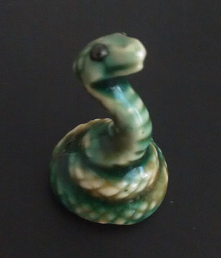
\includegraphics[scale=1]{ular-png}  
% 	\caption[Gambar {\it Serpentes} dalam format png]{Gambar {\it Serpentes} dalam format png} 
% 	\label{fig:ularpng} 
% \end{figure} 

% \dtext{19-20}
% \begin{figure}[H]
% 	\centering  
% 	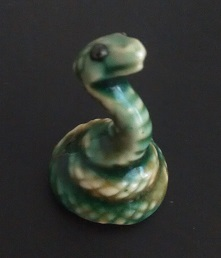
\includegraphics[scale=0.5]{ular-jpg}  
% 	\caption[Ular kecil]{Ular kecil} 
% 	\label{fig:ularjpg} 
% \end{figure} 
% \dtext{21-22}

% \begin{figure}[ht] 
% 	\centering  
% 	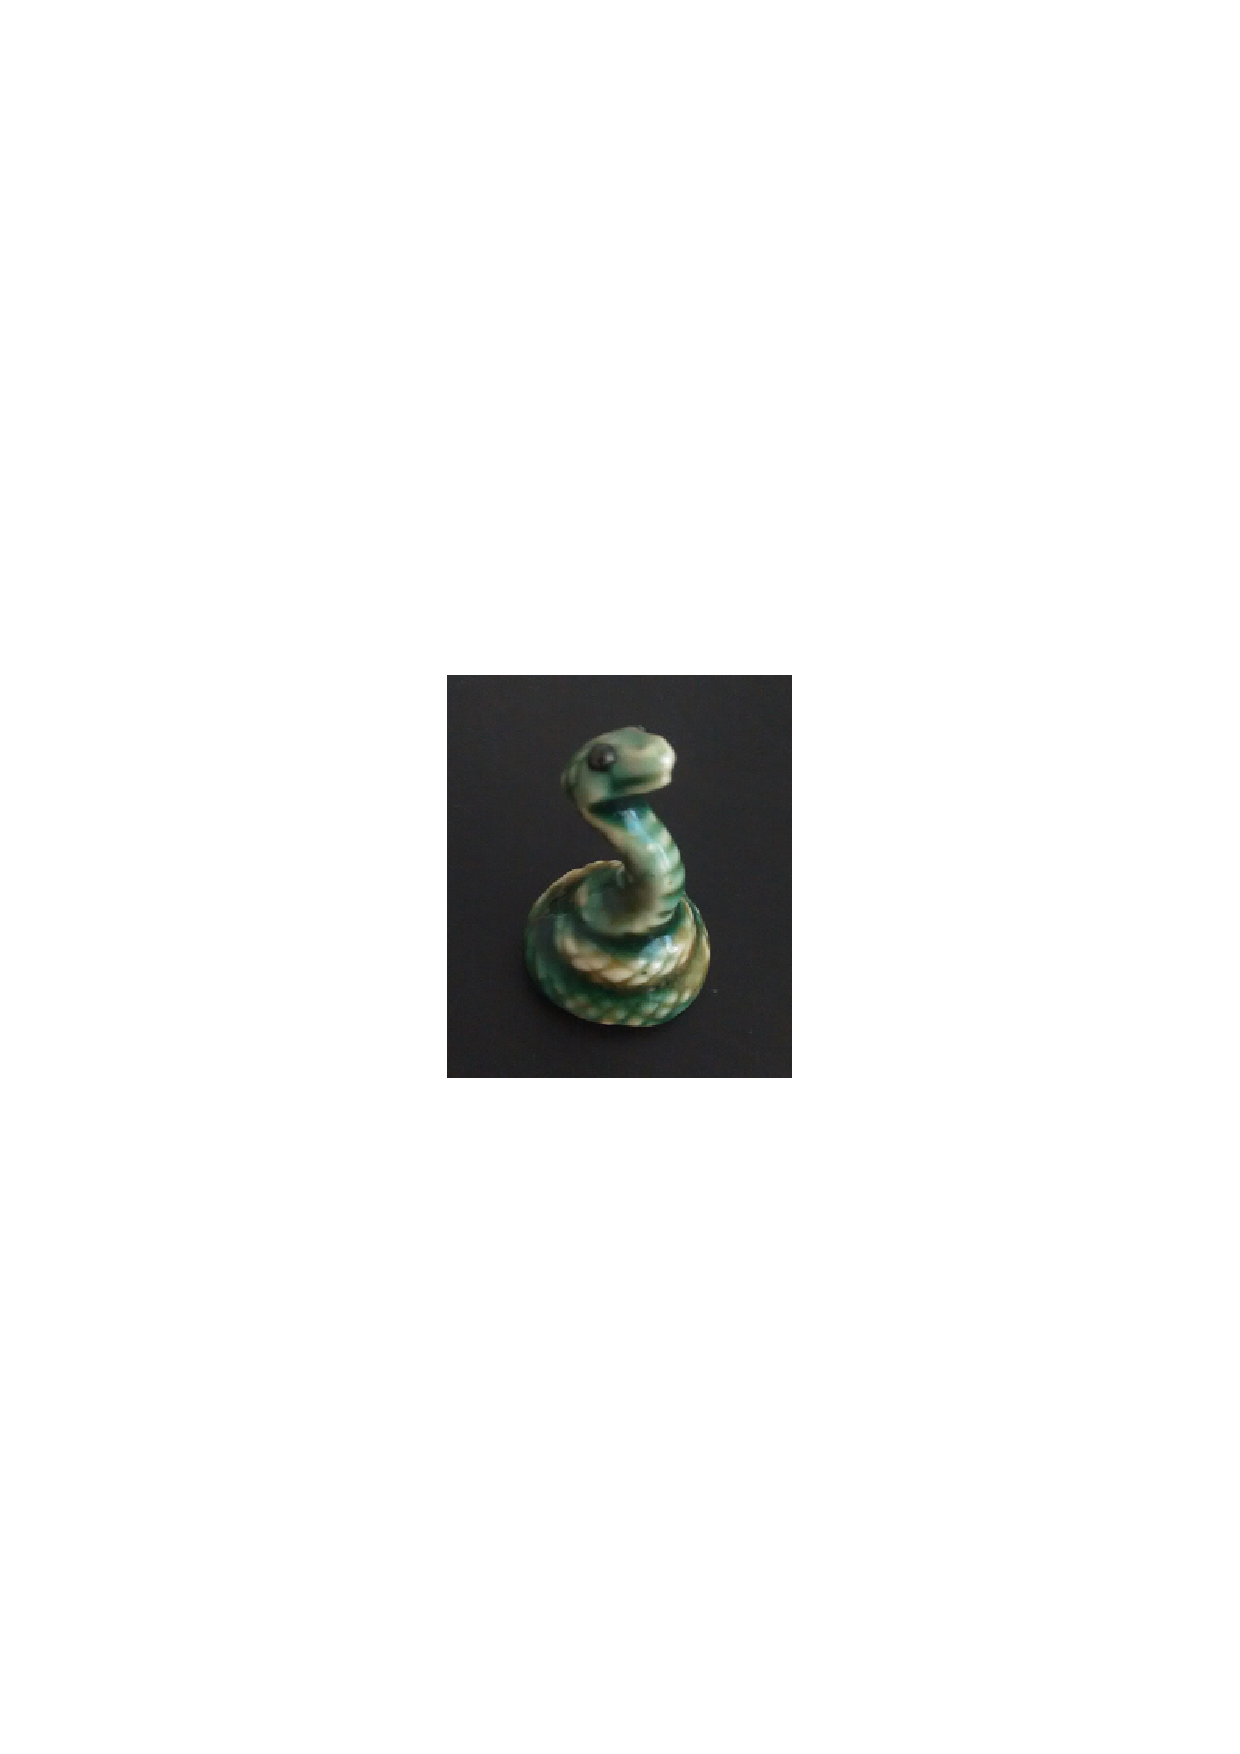
\includegraphics[scale=1]{ular-pdf}  
% 	\caption[ {\it Serpentes} betina]{ {\it Serpentes} jantan} 
% 	\label{fig:ularpdf} 
% \end{figure} 
 
